\documentclass{article}
\usepackage{graphicx} % Required for inserting images
\usepackage{tikz}
\usetikzlibrary{patterns} 
\usetikzlibrary{shapes}
\usepackage{pgfplots}
\usepackage{amsmath}
\pgfplotsset{compat=1.17}

\title{Készfeladat06.01}
\author{Viktor Soltész}
\date{November 2024}

\begin{document}

\maketitle

\section{Introduction}

 \tikz{ \draw (0,0)-- (1,0) (0,1)-- (1,1)
 (2,0.5) circle [radius=0.5] ; }

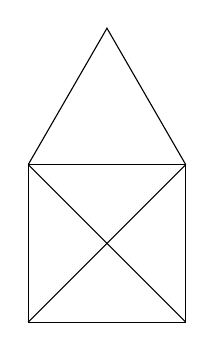
\begin{tikzpicture}[scale=2]
    \draw (0,0) rectangle (1,1);
    \draw (0,0) -- (1,1);
    \draw (0,1) -- (1,0);
    \draw (0,1)-- ++(60:1)--++(300:1);
\end{tikzpicture}
\tikz{\draw (0,0) -- (1,0) --(1,1) -- +(120:1)--(0,1)--(0,0)--(1,1)--(0,1)--(1,0)}

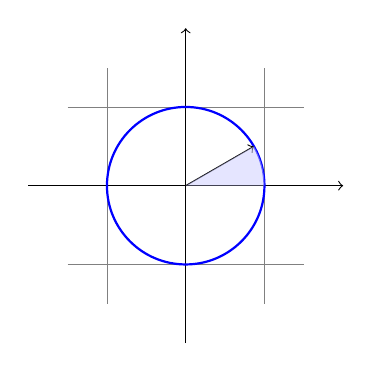
\begin{tikzpicture}
    \draw[very thin, gray] (-1.5,-1.5) grid (1.5,1.5);
    
    \draw[->] (-2,0) -- (2,0);
    \draw[->] (0,-2) -- (0,2);
    
    \draw[thick, blue] (0,0) circle (1);

    \draw[->] (0,0) -- ({cos(30)},{sin(30)});

    \fill[blue!20, opacity=0.5] (0,0) -- (1,0) arc (0:30:1) -- cycle;
    
\end{tikzpicture}

 \tikz{ \draw (0,0)-- ++(1,0)-- ++(72:1)-- ++(144:1)-- ++(216:1)-- cycle ;
 \draw (3,0)-- +(1,0)-- +(45:1)-- +(90:1)-- +(135:1)-- +(180:1) ; }


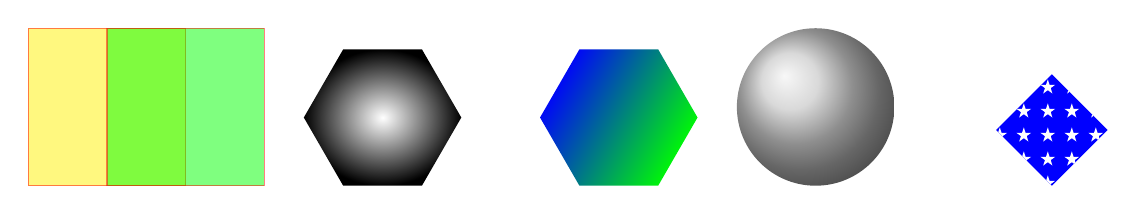
\begin{tikzpicture}
    \filldraw[draw=red,fill=yellow,opacity=0.5 ] (0,0) rectangle (2,2);
    \filldraw[draw=red, fill=green,opacity=0.5 ] (1,0) rectangle (3,2);

    \shade[shading=radial, outer color=black,
 inner color=white] ++(4,0)-- ++(1,0)-- ++(60:1)-- ++(120:1)-- ++(180:1)-- ++(240:1)-- cycle ;

     \shade[top color=blue, bottom color=green, shading angle=60] ++(7,0)-- ++(1,0)-- ++(60:1)-- ++(120:1)-- ++(180:1)-- ++(240:1)-- cycle ;

    \shade[shading=ball, ball color=black!20] (10,1) circle (1);

    \pattern[pattern=fivepointed stars, pattern color=white] ;

 \newcommand{\utvonalam}{++(13,0)-- ++(45:1)-- ++(135:1)-- ++(225:1)--cycle}
 \fill[blue] \utvonalam ;
 \pattern[pattern=fivepointed stars, pattern color=white] \utvonalam ;


\end{tikzpicture}



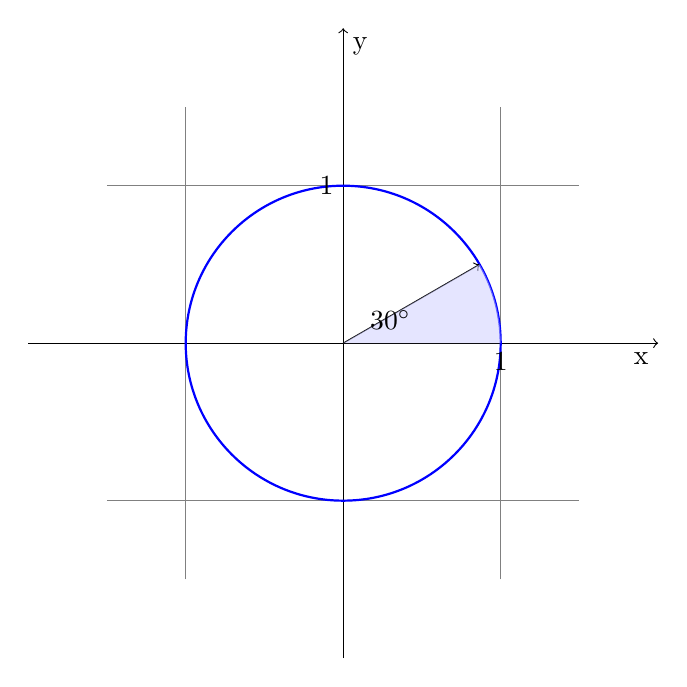
\begin{tikzpicture}[scale=2]
    \draw[very thin, gray] (-1.5,-1.5) grid (1.5,1.5);
    
    \draw[->] (-2,0) -- (2,0) node[below left]{x};
    \draw[->] (0,-2) -- (0,2) node[below right]{y};
    
    \draw[thick, blue] (0,0) circle (1);
    \node at (1,0) [below] {1};
    \node at (0,1) [left] {1};

    \draw[->] (0,0) -- ({cos(30)},{sin(30)});

    \fill[blue!20, opacity=0.5] (0,0) -- (1,0) arc (0:30:1) -- cycle;
    \node at (0.3,0.15) {$30^\circ$};
    
\end{tikzpicture}

\begin{tikzpicture}
    \draw (0,0) node [draw,shape=ellipse] (start) {START} ;
    \draw (0,-2) node [draw,shape=rectangle] (i) {$i \leftarrow 1$} ;
    \draw (0,-3) node [draw,shape=circle] (back) {} ;
    \draw (0,-5) node [draw,shape=diamond] (if) {$i \leq 10$} ;
    \draw (0,-7) node [draw,shape=rectangle] (print) {PRINT($i$)} ;
    \draw (0,-9) node [draw,shape=rectangle] (inc) {INC($i$)} ;
    \draw (0,-11) node [draw,shape=ellipse] (stop) {STOP} ;

    \draw[->] (start) -- (i);
    \draw[->] (i) -- (back);
    \draw[->] (back) -- (if);

    \draw[->] (if) -- node[ right] {igaz} (print);
    \draw[->] (print) -- (inc);
    \draw[->] (inc) to [out=0, in=0] (back);

    \draw[->] (if) to [out=180, in=180] node[left] {hamis} (stop);
\end{tikzpicture}


\end{document}
